\newpage
\section{More Playing with Blocks}\label{A:B2}
\index{base-ten blocks} 

Did you put your blocks away? Darn---there is still more to be
done! Just so that we are all on the same page, here are the basic
blocks:
\[
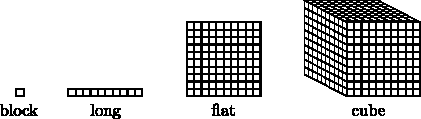
\includegraphics{../graphics/baseTenBlocks.pdf}
\]

\begin{prob}
Now Oscar is modeling the basic multiplication algorithm:
\[
\begin{tabular}{@{}r@{}}
11~~\\
234\\
$\times$~~3\\ \hline
702
\end{tabular}
\]
\[
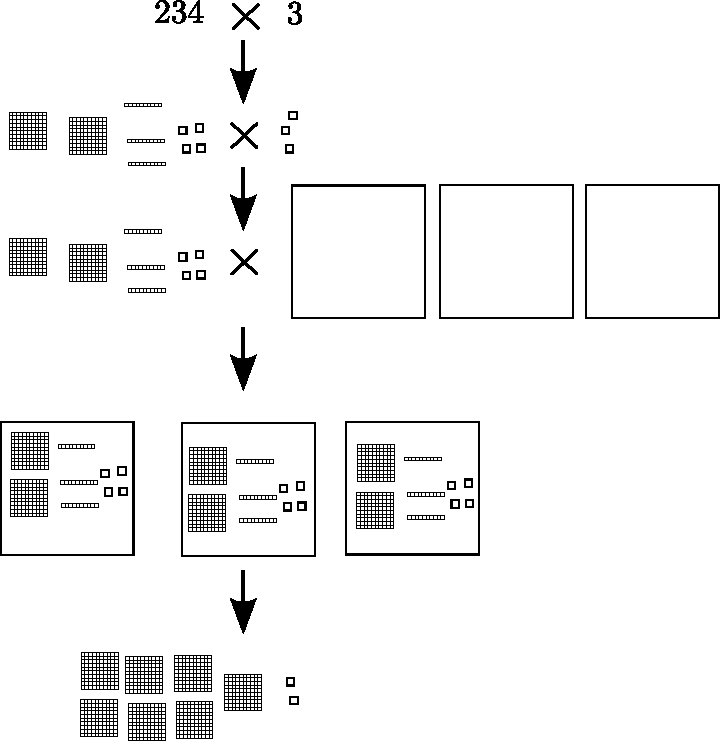
\includegraphics{../graphics/oscarMult.pdf}
\]
Can you explain what is going on? What do you think of his model?
\end{prob}




\begin{prob}
Here is an example of the basic division algorithm:
\[
3\,\begin{tabular}[b]{@{}r@{}r} 
67 &\, R$1$\\ 
\cline{1-1}
\big)\begin{tabular}[t]{@{}l@{}} 202\\ 
18 \\ 
\divrule{0}{2}  ~22 \\
 ~21\\
 \divrule{1}{2}
~~1
\end{tabular}
\end{tabular}
\]
Explain how to model this algorithm with base-ten blocks.
\end{prob}



